%%%%%%%%%%%%%%%%%%%%%%%%%%%%%%%%%%%%%%%%%%%%%%%%%%
% CODE SNIPPETS
%%%%%%%%%%%%%%%%%%%%%%%%%%%%%%%%%%%%%%%%%%%%%%%%%%
\newpage

% CROSS-REFERENCES
\section*{Cross-References}
\noindent ref: \ref{ch:introduction} % number

\noindent autoref: \autoref{ch:introduction} % name and number

\noindent pageref: \pageref{ch:introduction} % page number

\noindent autopageref: \autopageref{ch:introduction} % page name and number

% ch:chapter
% sec:section
% subsec:subsection
% fig:figure
% tab:table
% eq:equation
% lst:code-listing
% itm:enumerated-list-item
% alg:algorithm
% app:appendix-subsection

% CITATIONS
\section*{Citations}
\noindent textcite: \textcite[p. 13]{westfahl:space}

\noindent textcites: \textcites[p. 13]{westfahl:space}{angenendt}[p. 13]{baez/article}

\noindent parencite: \parencite[see][p. 13]{westfahl:space}

\noindent parencites: \parencites(see)(and \autoref{ch:introduction})[p. 13]{westfahl:space}{angenendt}[p. 34]{baez/article}

% ABBREVIATIONS
\section*{Abbreviations}
\noindent gls: \gls{abbr} % singular

\noindent Gls: \Gls{abbr} % singular capitalised

\noindent glspl: \glspl{abbr} % plural

\noindent Glspl: \Glspl{abbr} % plural capitalised

% FOOTNOTES
\section*{Footnotes}
Lorem ipsum dolor sit amet, consectetur adipiscing elit\footnote{Ut enim ad minim veniam, quis nostrud exercitation ullamco laboris nisi ut aliquip ex ea commodo consequat. Duis aute irure dolor in reprehenderit in voluptate velit esse cillum dolore eu fugiat nulla pariatur.}, sed do eiusmod tempor incididunt ut labore et dolore magna aliqua. Ut enim ad minim veniam, quis nostrud exercitation ullamco laboris nisi ut aliquip ex ea commodo consequat. Duis aute irure dolor in reprehenderit in voluptate velit esse cillum dolore eu fugiat nulla pariatur.\footnote[42]{...is that the answer to everything?}

% ITEMIZE
\section*{Itemize}
\begin{itemize}
    \item Lorem ipsum dolor sit amet, consectetur adipiscing elit, sed do eiusmod tempor incididunt ut labore et dolore magna aliqua.
    \item Ut enim ad minim veniam, quis nostrud exercitation ullamco laboris nisi ut aliquip ex ea commodo consequat.
\end{itemize}

% ENUMERATE
\section*{Enumerate}
\begin{enumerate}
    \item Lorem ipsum dolor sit amet, consectetur adipiscing elit, sed do eiusmod tempor incididunt ut labore et dolore magna aliqua.
    \item Ut enim ad minim veniam, quis nostrud exercitation ullamco laboris nisi ut aliquip ex ea commodo consequat.
\end{enumerate}

% LISTINGS
\section*{Listing}
Lorem ipsum dolor sit amet, \lstinline[style=python]{first_name = "Nora"} consectetur adipiscing elit, sed do eiusmod tempor incididunt ut labore et dolore magna aliqua.

\begin{lstlisting}[style=python]
# This is some sample python code
first_name = "Nora"
favorite_language = "Python"
print(f"Hi, my name is {first_name}. I am learning {favorite_language}.")
\end{lstlisting}

% FIGURE
\section*{Figure}
\begin{figure}[H]
\ffigbox[\textwidth]
    {\caption{Caption}\label{fig:label-1}}
    {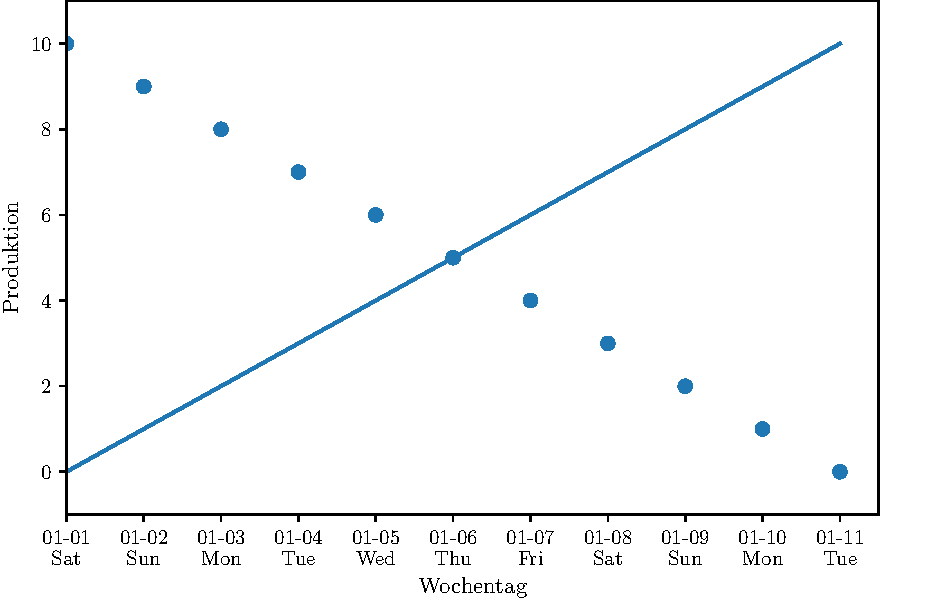
\includegraphics[width=\hsize]{Resources/figure.pdf}
    \floatfoot{Floatfoot.}}
\end{figure}

% TABLE
\section*{Table}
\begin{table}[H]
\ttabbox
    {\caption{Caption}\label{tab:label-1}}
    {\begin{tabular}{@{}cl*{2}{S[table-format=+2.2, round-mode=places, round-precision=2]}l@{}} \toprule
        & & \multicolumn{3}{c}{Measurements} \\ \cmidrule(l){3-5}
        & {Weekday} & {Temperature} & {Percipitation} & {Cloudy} \\ \midrule
        \csvreader[late after line=\\, head to column names, filter={\thecsvinputline<9}]{Resources/data.csv}{}{\thecsvrow & \weekday & \temperature &\percipitation & \cloudy} \midrule
        \csvreader[late after line=\\, head to column names, filter={\thecsvinputline=9}]{Resources/data.csv}{}{& \weekday & \temperature &\percipitation & \cloudy} \bottomrule
    \end{tabular}
    \floatfoot{Floatfoot.}}
\end{table}

% NOTE: \csvautobooktabular{Resources/data.csv} creates automatic table
% NOTE: \thecsvrow returns row number after filter, \thecsvinputline returns row number before filter
% NOTE: \csvcoli is based on roman numerals i.e. it continues at csvrowiv, csvrowv, etc.
% NOTE: if csvsimple cannot find the header of the first column, this is likeley due to LaTeX not ignoring the utf-8 BOM byte order mark U+FEFF: try switching to a different compiler such as XeLaTeX or LuaLaTeX

% FLOATROW
\section*{Floatrow}
\begin{figure}[H]
    \begin{floatrow}
    \ffigbox[\hsize]
        {\caption{Caption}\label{fig:label-2}}
        {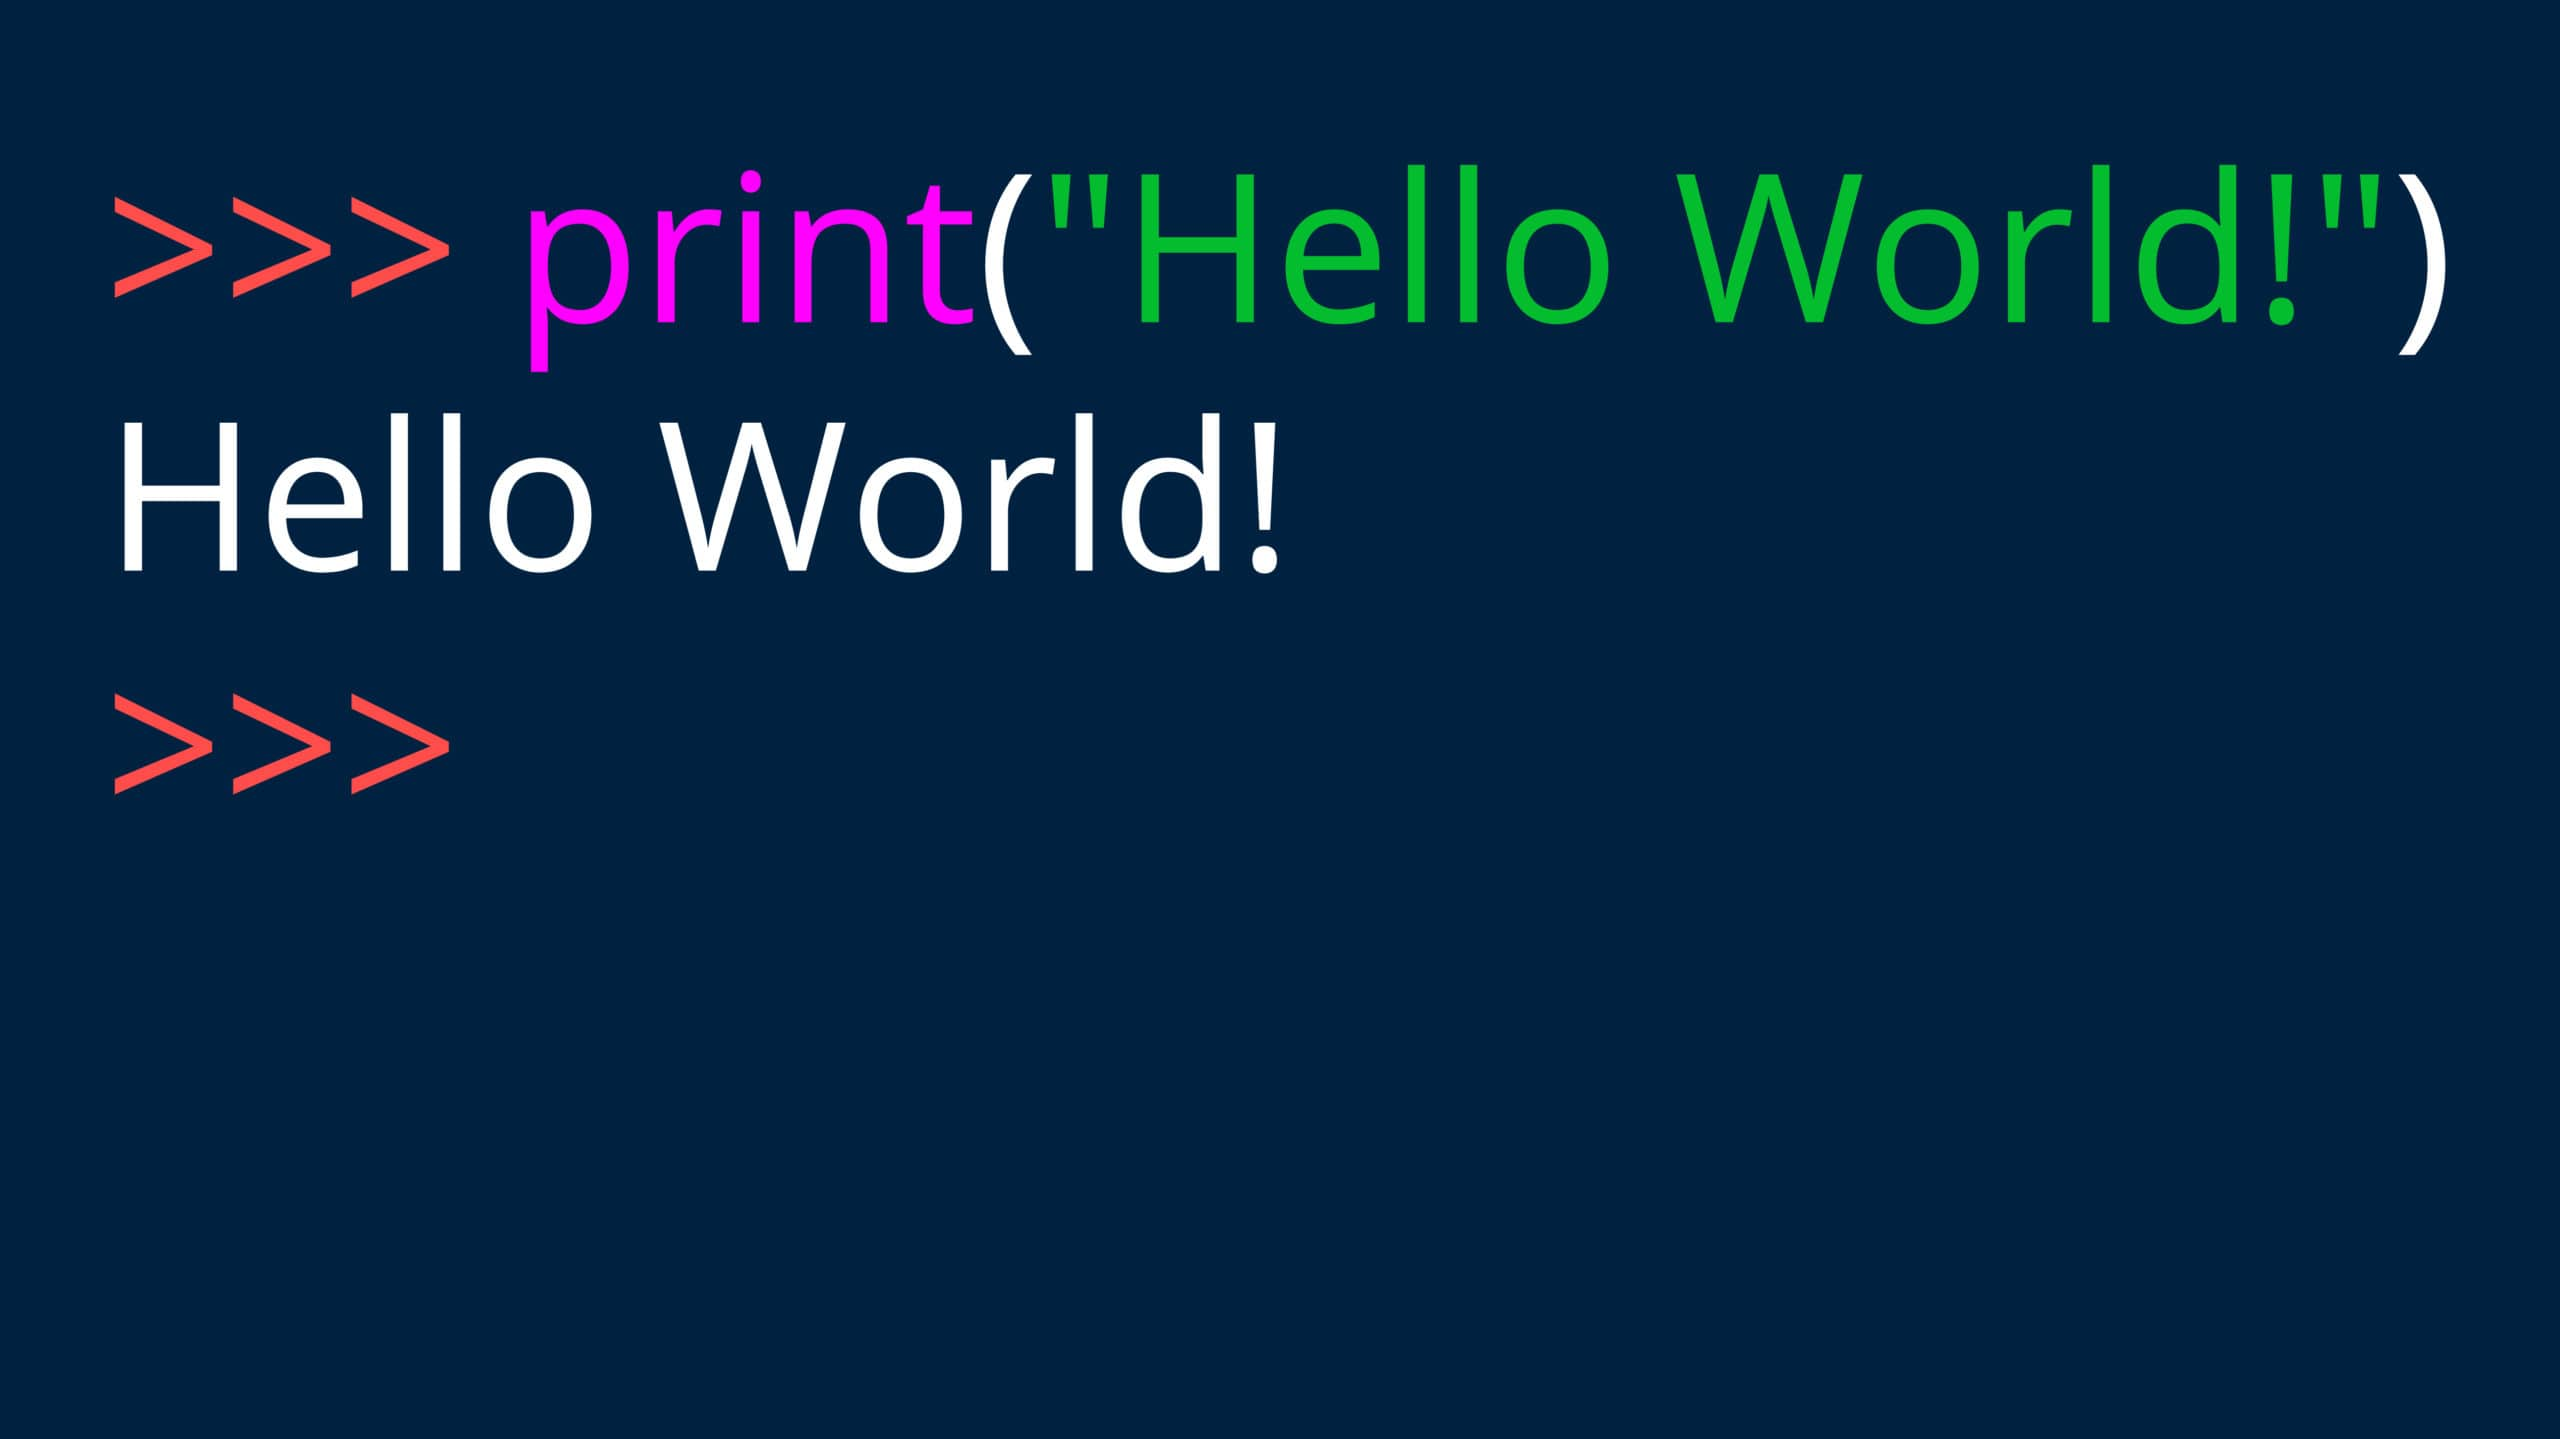
\includegraphics[width=\hsize]{Resources/image.jpeg}
        \floatfoot{Floatfoot.}}
    \ttabbox[\hsize]
        {\caption{Caption}\label{tab:label-2}}
        {\begin{tabular}{@{}lS[table-format=5]S[table-format=3.2]@{}} \toprule
            Datensatz & {Länge (n)} & {Länge (\%)} \\ \midrule % braces escape siunitx formatting
            Training    & 9999  & 99.99 \\
            Validierung & 9999  & 99.99 \\
            Test        & 9999  & 99.99 \\ \midrule
            Total       & 10000 & 100.00 \\ \bottomrule
        \end{tabular}
        \floatfoot{Floatfoot.}}
    \end{floatrow}
\end{figure}